\chapter{Two-Dimensional SEAS Model}
\label{chap:2DSEAS}
From now on, we consider the SEAS problem in a 2D domain with a 1D fault where displacements, slip rates and stresses are orthogonal to the plane. The model is described in \autoref{sec:2DSEAS__BP1Problem}, followed by the method to solve the 2D domain in \autoref{sec:2DSEAS__DG} and finally \autoref{sec:2DSEAS__EvolutionOfQuantities} gives an insights on how the system evolves with time.

\section{BP1 Benchmark Problem}
\label{sec:2DSEAS__BP1Problem}
Erickson et al. \cite{BP1-Benchmark} proposed the BP1 benchmark problem based on the SEAS model of \cite{GeneralSEASSimulations}, which is a 2D antiplane problem with a 1D vertical fault. This means that the domain is an orthogonal surface to the real fault and only shear stress and displacements out of the plane are considered. A schematic view of the model is given in \autoref{fig:2DSEASModel}. \\ 

\begin{figure}[H]
	\centering
	\begin{subfigure}[t]{0.49\textwidth}
		\centering
		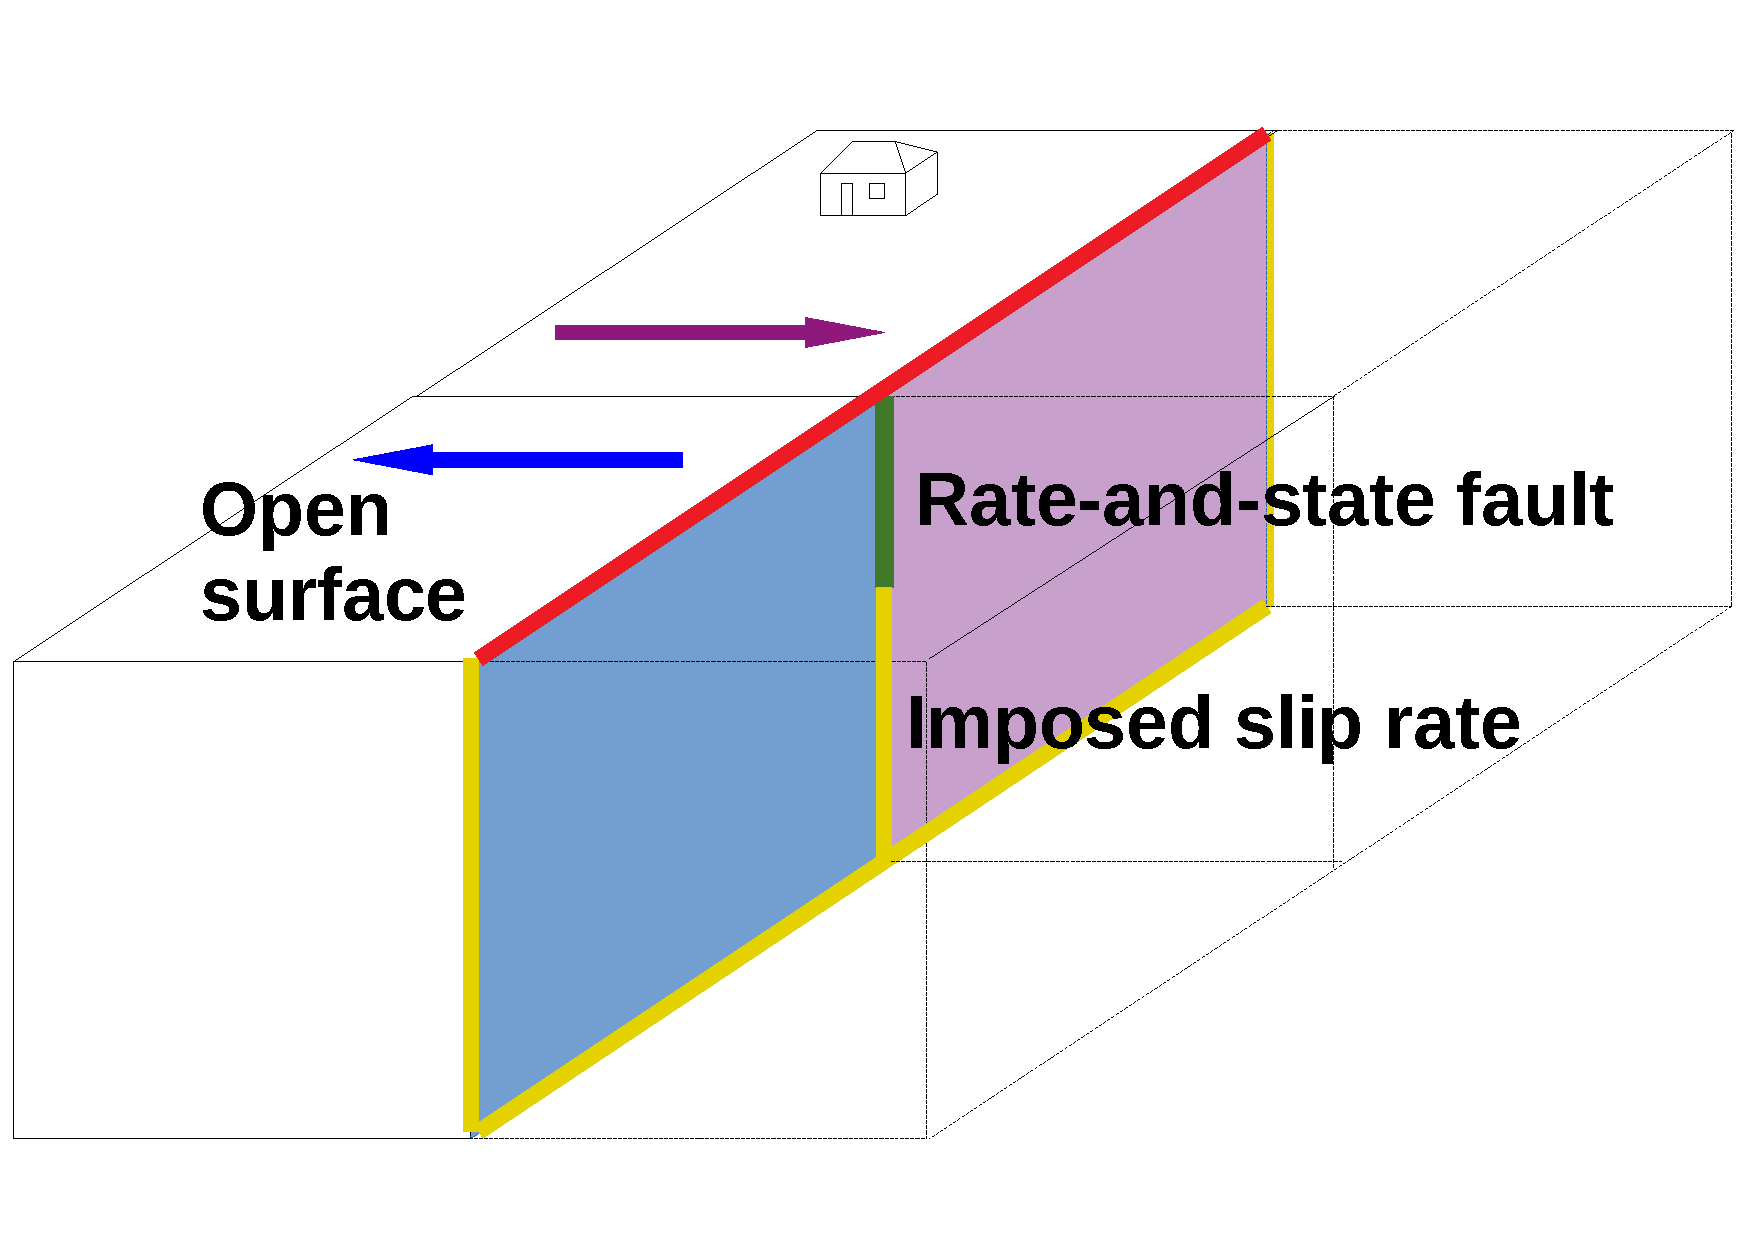
\includegraphics[height=4.7cm]{images/SEAS_2D_picture.pdf}
		\subcaption{Initial condition \\ \ }
	\end{subfigure}
	\begin{subfigure}[t]{0.49\textwidth}
		\centering
		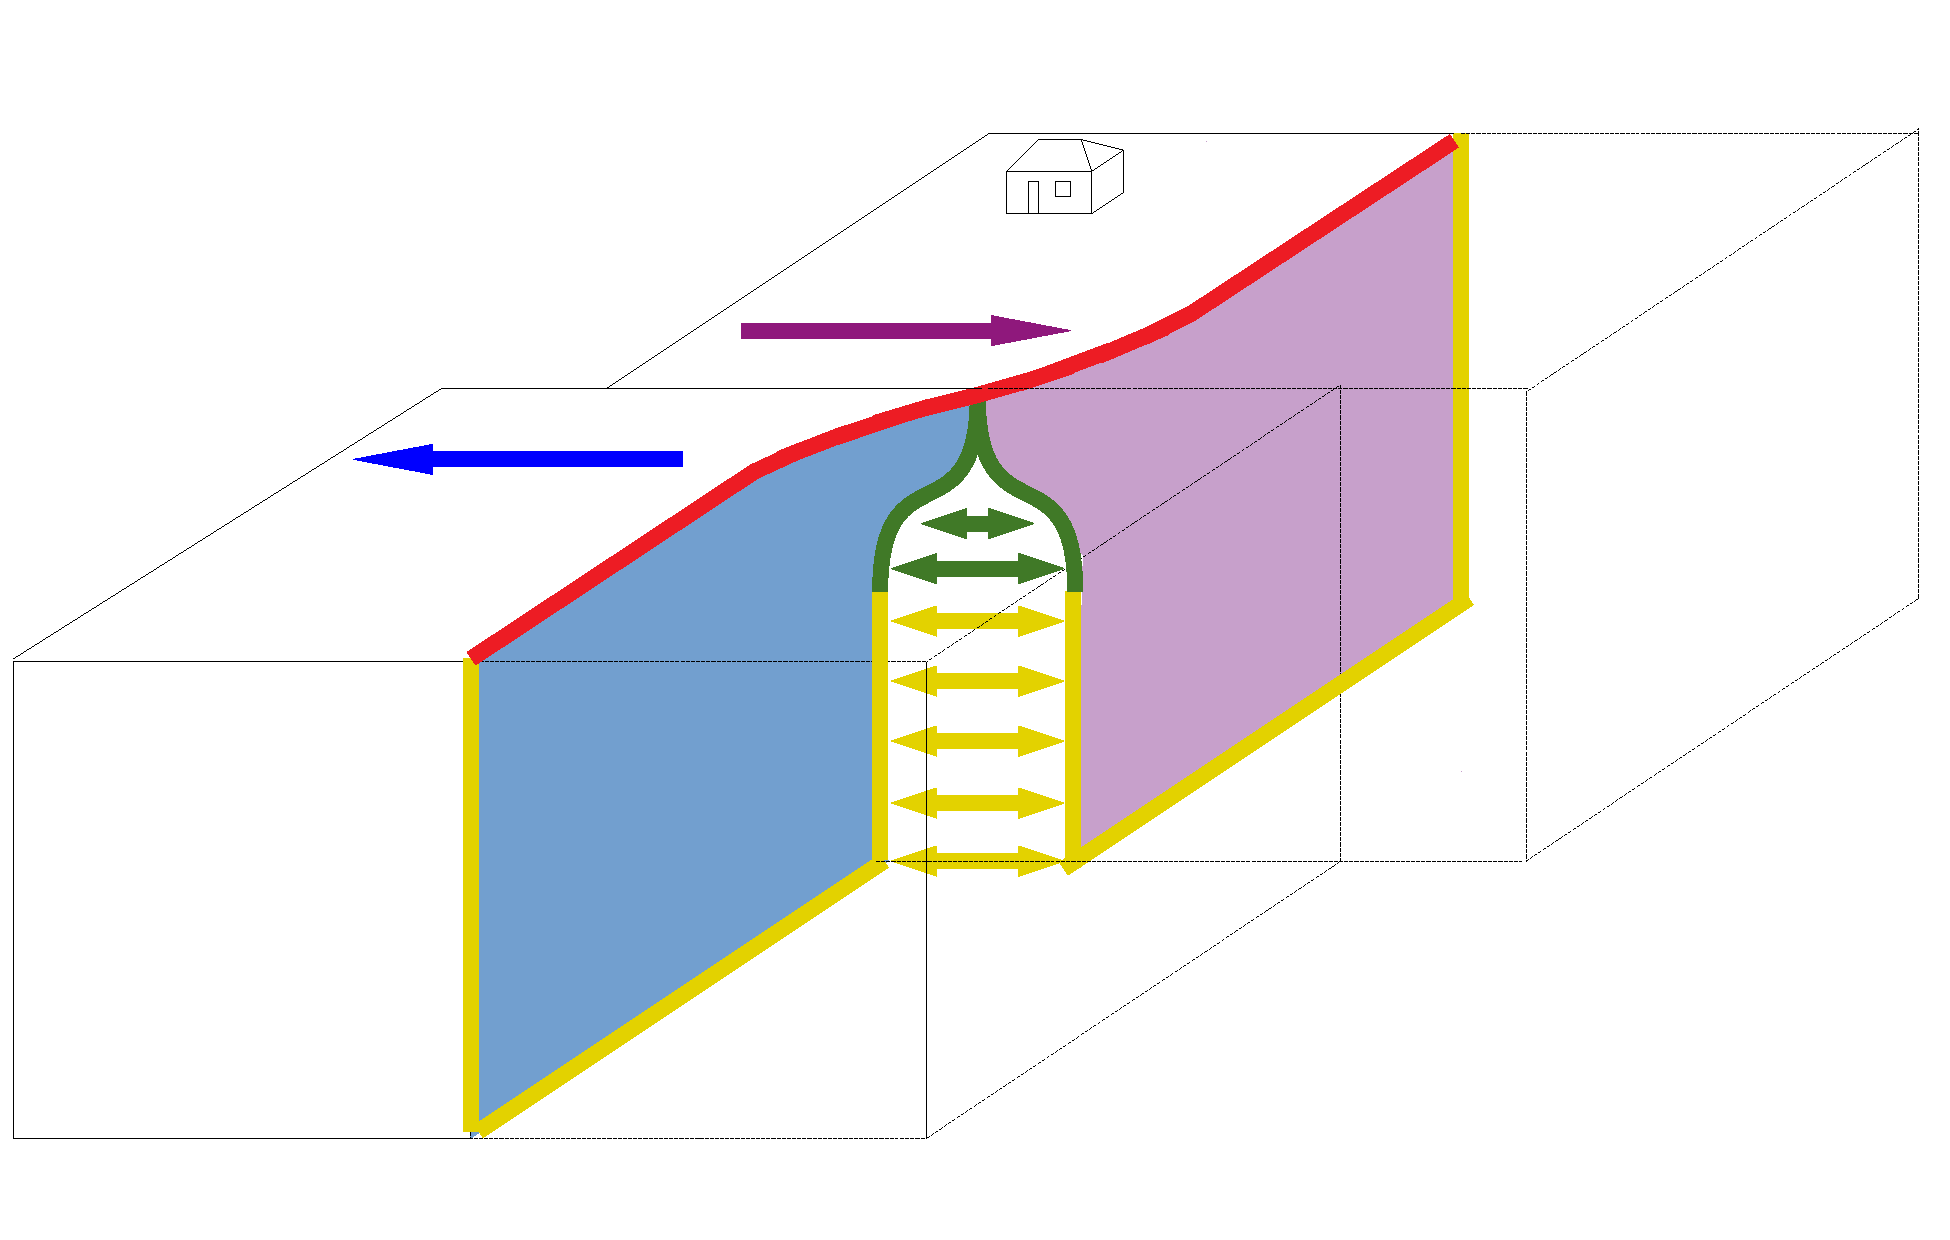
\includegraphics[height=4.7cm]{images/SEAS_2D_picture_after_slip.pdf}
		\subcaption{After some slip, before the first \\ earthquake}
	\end{subfigure}
	\caption{Illustration of the 2D SEAS model with two tectonic plates. The domain is compound of the blue and purple surfaces. Since both plates move in opposite directions, the slip, shown as arrows in the right picture, increases and the domain deforms.}
	\label{fig:2DSEASModel}
\end{figure}
It consists of two square, symmetric tectonic plates that are pulled in opposite directions by an environment slip rate $V_p/2=5\cdot10^{-10}$m/s, applied as Dirichlet condition on the yellow boundary of the domain. On the red boundary, there is the traction-free open surface which translates into Neumann boundary conditions. Finally, the most interesting section of the domain is the rate-and-state fault on the green boundary. It is driven by the rate-and-state friction with Dieterich-Ruina ageing discussed in \autoref{ssec:FrictionLaws} and describes the transition from the bottom of the fault, where the slip increases linearly in time, to the top, which does almost not move in the aseismic phase and recovers the accumulated delay by a sudden increase in slip during an earthquake. \\

As the out-of-plane component $u$ is the only non-zero component of the displacement vector, the elasticity equation reduces to a Poisson problem. Indeed, the Cauchy stress tensor $\mathbf{\sigma}$ from \autoref{eq:CauchyStressTensor} is zero except for the component $\tau_{xy}$ and only the components $\mathbf{C_{xyzx}}$ and $\mathbf{C_{xyzy}}$ of the material tensor remain, both set to $\mu$. The governing equations are stated in \autoref{eq:Poisson_problem_2D}, where the $x_i$ denote a position in the spatial directions $x$ and $y$ for $i=1,2$ and $n$ is the normal vector of the open surface, usually  $n=(0,1)^T$.
\begin{equation}
	\label{eq:Poisson_problem_2D}
	\begin{cases}
		-\pdv{}{x_i}\left(\mu\pdv{u}{x_i}\right) = 0 & \text{in } \Omega \\
		\qquad\qquad\quad  u = V_pt/2 & \text{on the imposed slip rate } \Gamma_D \\
		\qquad\ \ \, \mu\pdv{u}{x_i}n_i = 0 & \text{on the open surface } \Gamma_N \\
		\qquad\qquad\  \llbracket u \rrbracket = S  & \text{on the rate-and-state fault } \Gamma_F
	\end{cases}
\end{equation}

The slip $S$ on the rate-and-state fault is the difference between the displacements of the two tectonic plates at the same fault node. Since we solve for symmetric domains, the displacements are identical but in opposite directions, we thus have $S = \llbracket u \rrbracket = u^+ - u^- = 2u$. Further, on the rate-and-state fault we have to solve for the slip $S$ and the state variable $\psi$ over time in a DAE stated in \autoref{eq:DAEFormulation2DSEAS} on each fault node $i$. 
\begin{equation}
	\label{eq:DAEFormulation2DSEAS}
	\begin{cases}
		\,\  0 = F_i(U,S,\psi,V) = \tau_i(U,S) - a\sigma_n\text{arsinh}\left(\frac{V_i}{2V_0}e^{\frac{\psi_i}{a}}\right) -\eta V_i & \text{(Friction law)}\\
		\dot{\psi_i} = G_i(\psi_i, V_i) =\frac{bV_0}{L}\left(e^{\frac{f_0-\psi_i}{b}} - \frac{V_i}{V_0}\right) & \text{(Ageing law)} \\
    	\dot{S_i} = V_i & \text{(Slip rate)}
	\end{cases}
\end{equation} 
The traction term $\tau_i$  is the sum of the shear stress orthogonal to the fault $\mu\pdv{u}{x_i}n_i$ (here $n_i = (1,0)^T$) and a constant pre-stress $\tau_0$. The DAE above is the core problem of the next chapter. 

\section{Formulation of the discontinuous Galerkin method}
\label{sec:2DSEAS__DG}
The 2D domain is discretized by an unstructured grid with a high resolution around the rate-and-state fault and a coarser resolution in the remaining domain. An example grid with 200 fault elements is shown in \autoref{fig:mesh_BP1_200_fault_elements}.

\begin{figure}[H]
	\centering
	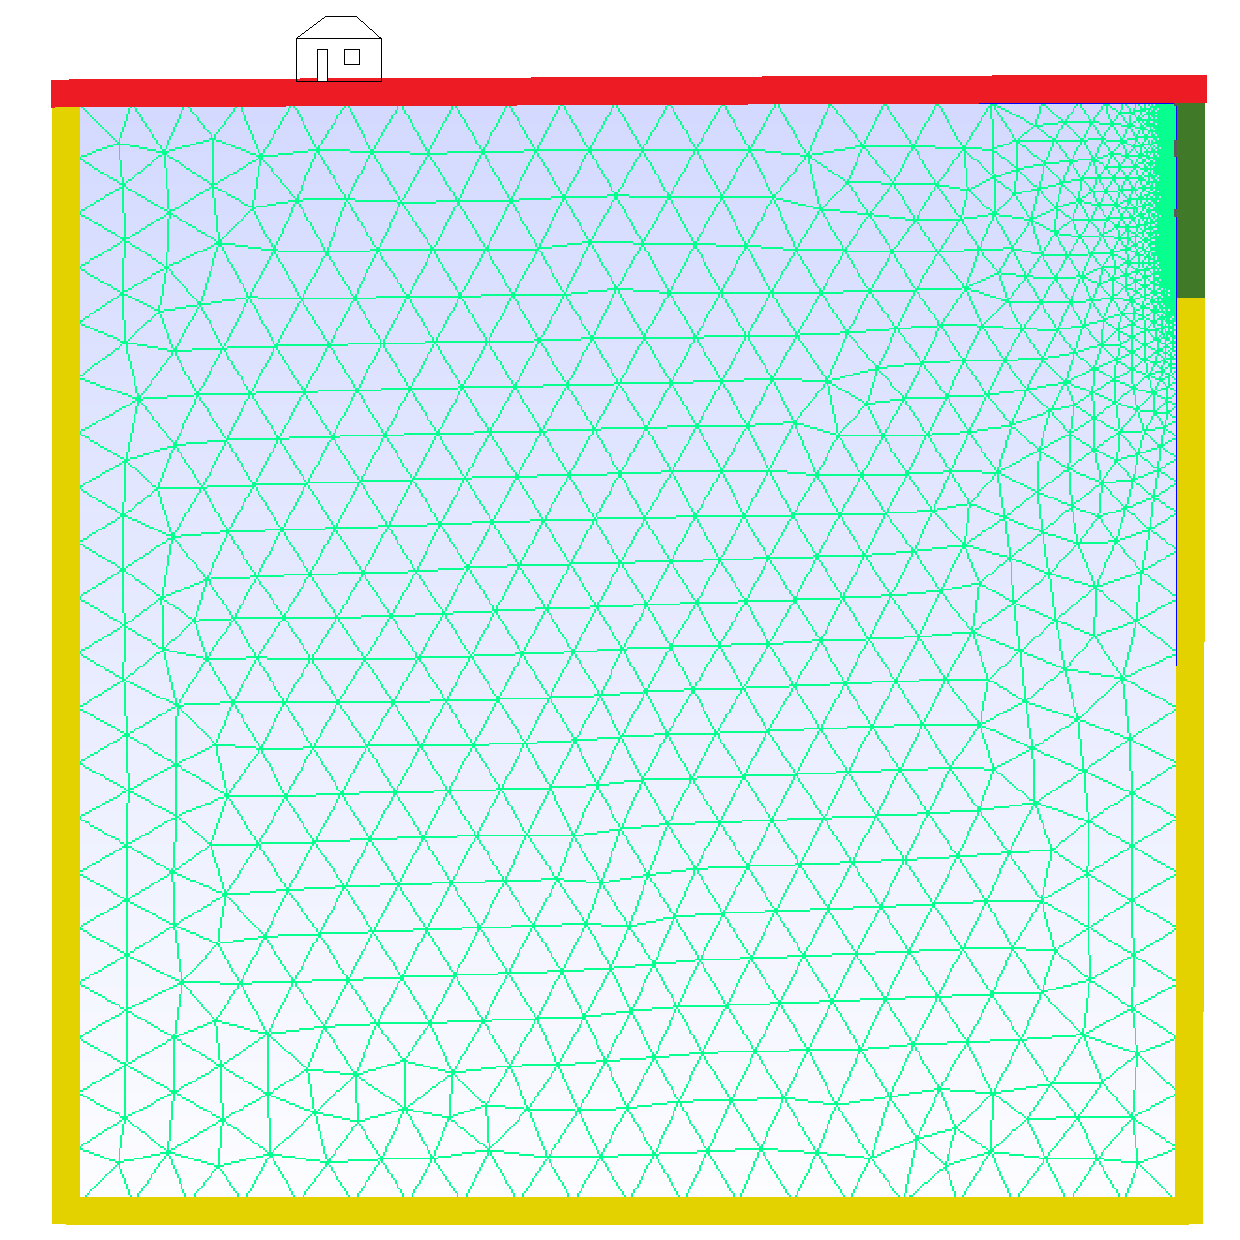
\includegraphics[width=0.4\textwidth]{images/BP1_mesh_with_boundaries.pdf}
	\caption{Space discretization of the BP1 problem with 200 elements on the fault}
	\label{fig:mesh_BP1_200_fault_elements}
\end{figure}

The elliptic Poisson problem $-\Delta u = f$ with mixed Dirichlet and Neumann boundary conditions is solved with the discontinuous Galerkin (DG) method described by Rivière \cite{DG-elliptic-problems}. The problem is first transformed into its first order weak form and the domain discretized into triangular elements. To integrate an edge exactly with polynomial basis functions of order $k$, $k+1$ nodes are needed on the edge. In this thesis we only consider the case $k=2$, such that the number of fault nodes is always three times the number of fault elements and all relevant quantities for the time integration ($V$, $S$ and $\psi$) are evaluated on these nodes. To obtain the displacement $u_i$ at each node in $\Omega$, a matrix $\mathbf{A}$ can be assembled \cite{DG_for_SEAS} such that:
\begin{equation}
	\mathbf{A}u = b(S)
\end{equation}
The matrix $\mathbf{A}$ does not depend on the displacement or any other variable, its LU-decomposition can therefore be precomputed and solving for the displacement only involves one forward and one backward substitution. The right-hand side $b$ includes all boundary conditions, especially from the slip at the rate-and-state fault, and therefore changes over time.


\section{Evolution of the slip, the slip rate and the state variable}
\label{sec:2DSEAS__EvolutionOfQuantities}
\autoref{fig:EvolutionAllQuantitiesMinMaxStacked200Elements} gives a first insight into the evolution of the characteristic quantities $S$, $\psi$ and $V$ in the rate-and-state fault over time. The maximum slip increases linearly over time, it occurs at the bottom of the friction area in the fault at the transition to the imposed slip rate. The minimum slip occurs close to the surface, where nothing moves until an earthquake suddenly shifts the open surface. Each earthquake is accompanied by a peak in the maximum slip rate $\max_i(V_i)$ of up to $5$m/s, which usually remains below $10^{-9}$m/s in the aseismic phase. The state variable $\psi$ at the open surface approaches $0.8$ during the aseismic phase until an earthquake provokes a sudden drop to $0.4$. For the BP1 benchmark an accurate prediction of the period between earthquakes is a critical metric, this naturally requires an accurate evaluation of the aseismic phase but also of the earthquake phase, as the simulated slip increase at the open surface directly affects the duration until the next earthquake.

\begin{figure}[H]
	\centering
	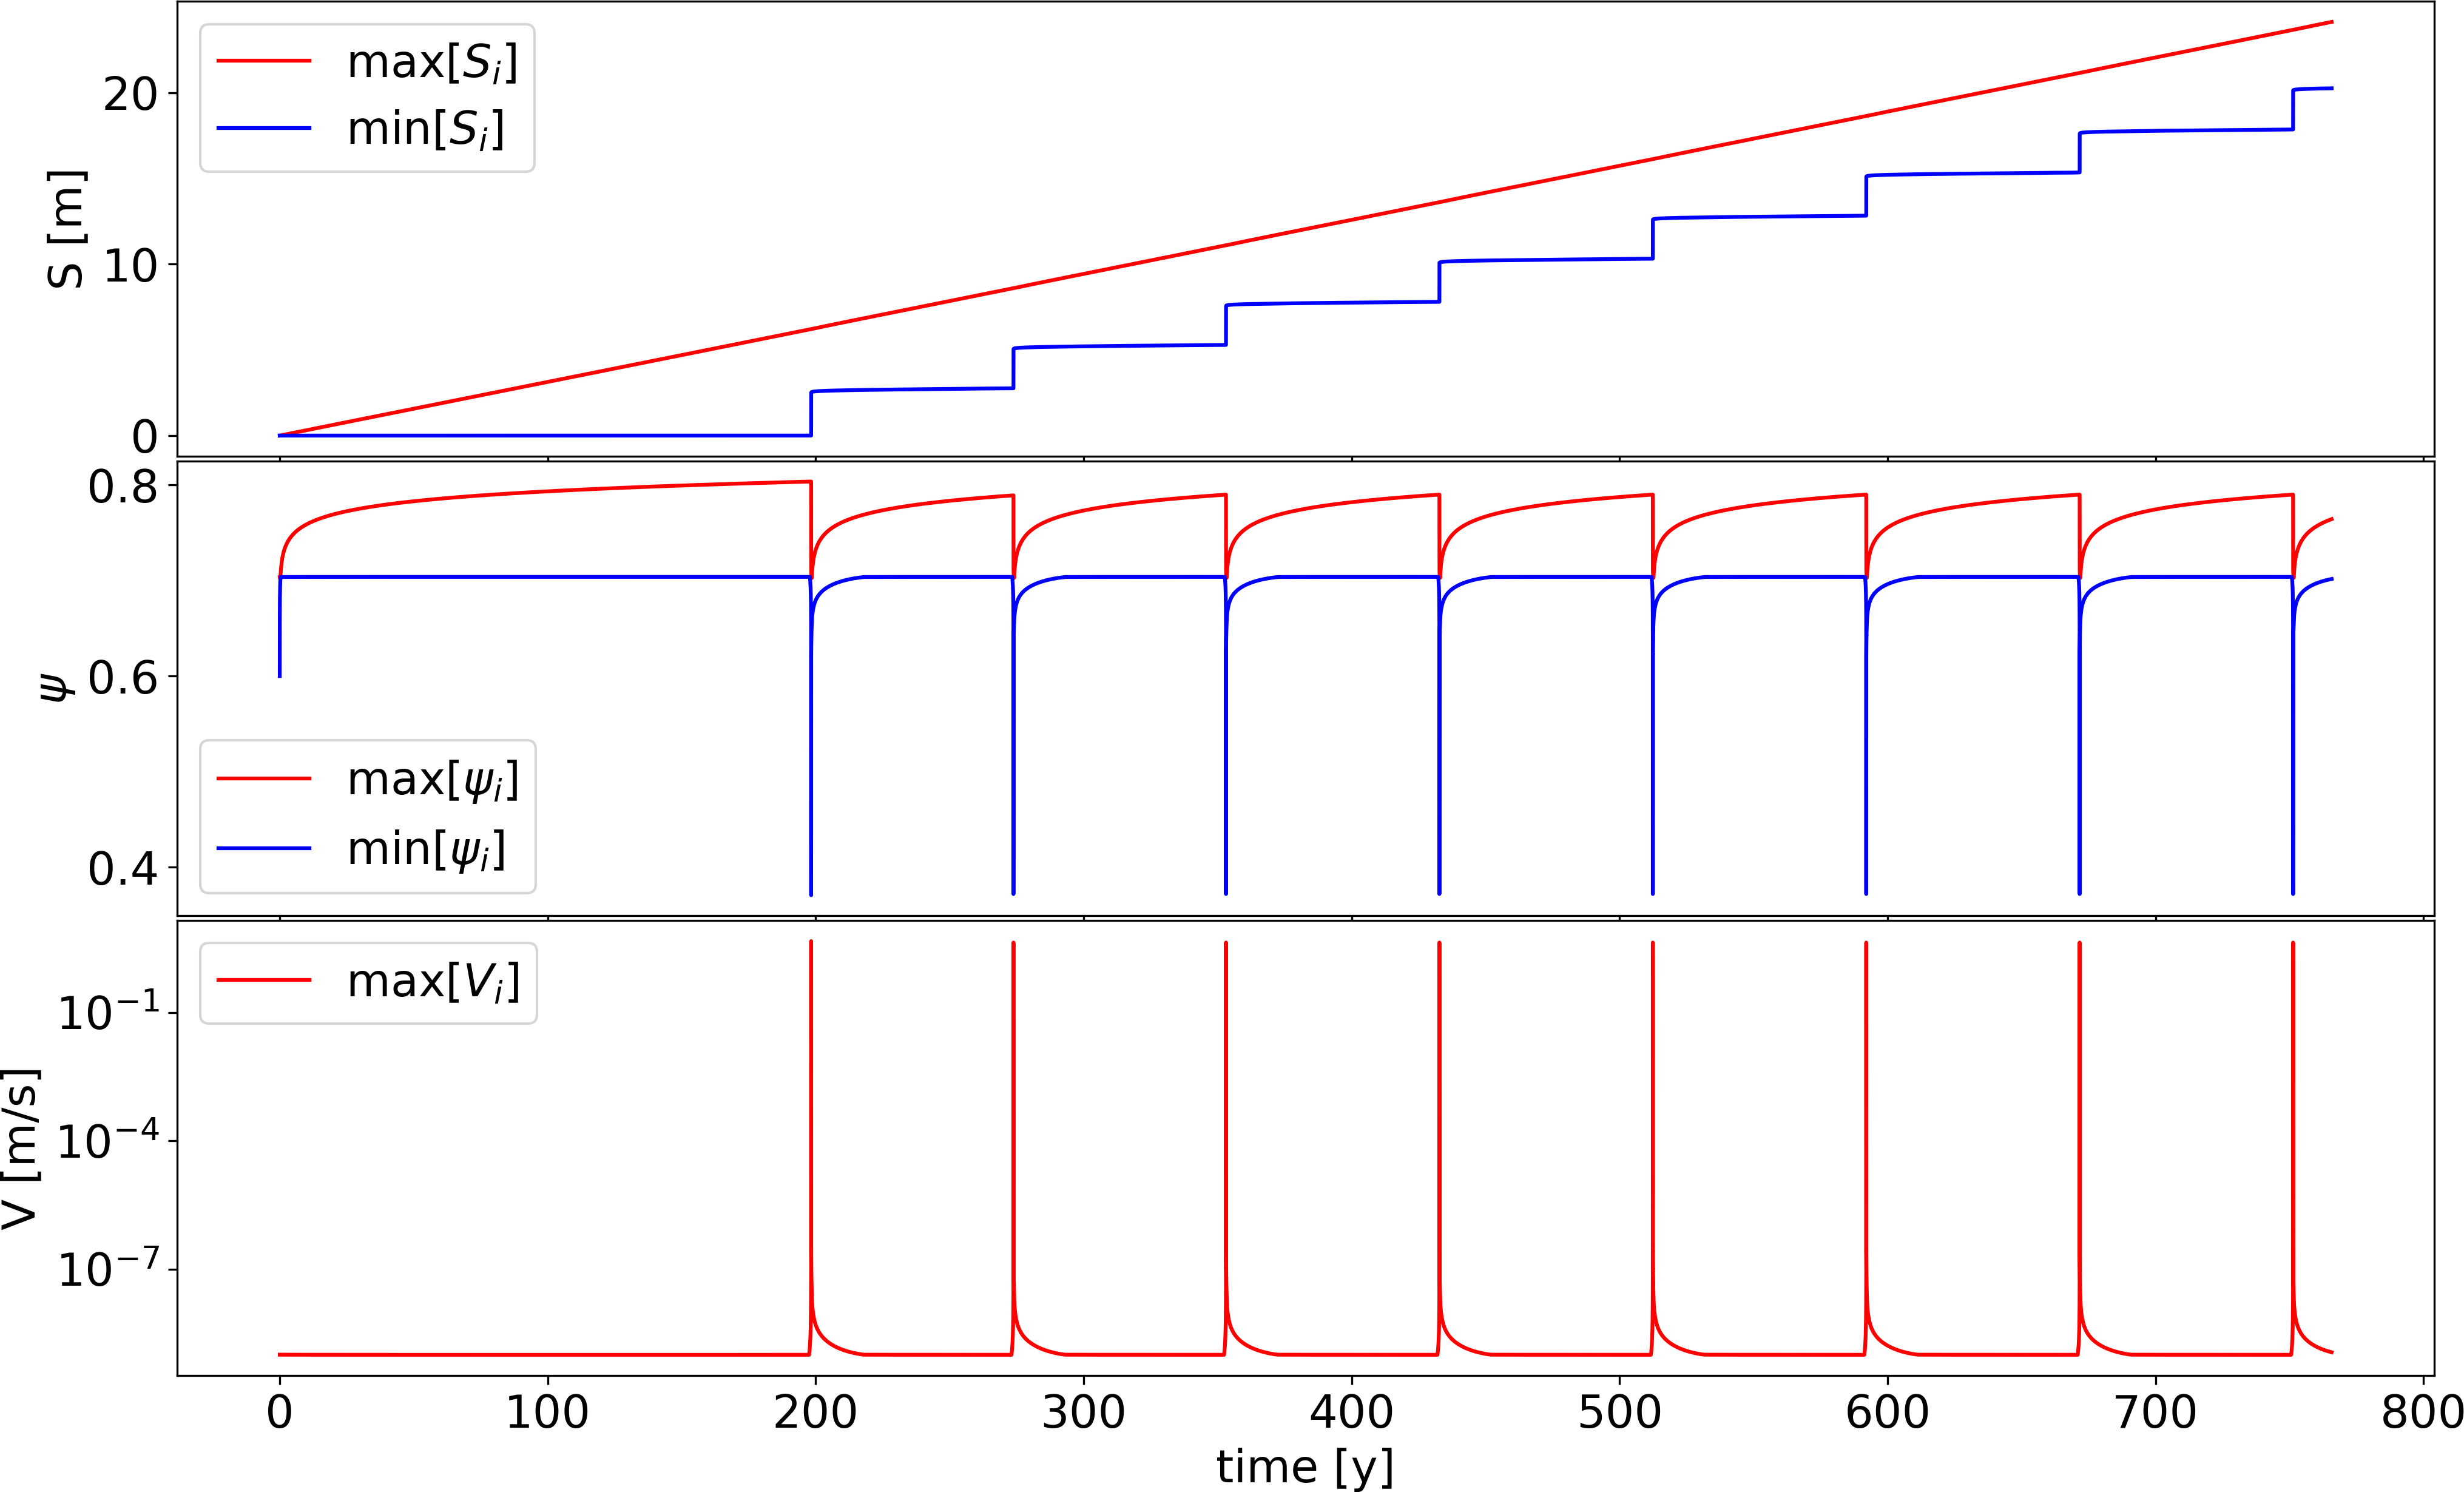
\includegraphics[width=0.7\textwidth]{images/TANDEMtimeEvolution_MinMaxAllStacked_Size200_RKDP5_extendedODE.png}
	\caption{Evolution of the slip $S$, the state variable $\psi$ and the slip rate $V$ over 770 years on a domain with 200 fault elements}
	\label{fig:EvolutionAllQuantitiesMinMaxStacked200Elements}
\end{figure}

A fine mesh resolution at the fault is essential for an accurate prediction of earthquake events. \autoref{fig:EvolutionAllQuantitiesScalability} depicts the slip at the open surface and the maximum slip rate for vary-

\begin{figure}[H]
	\centering
	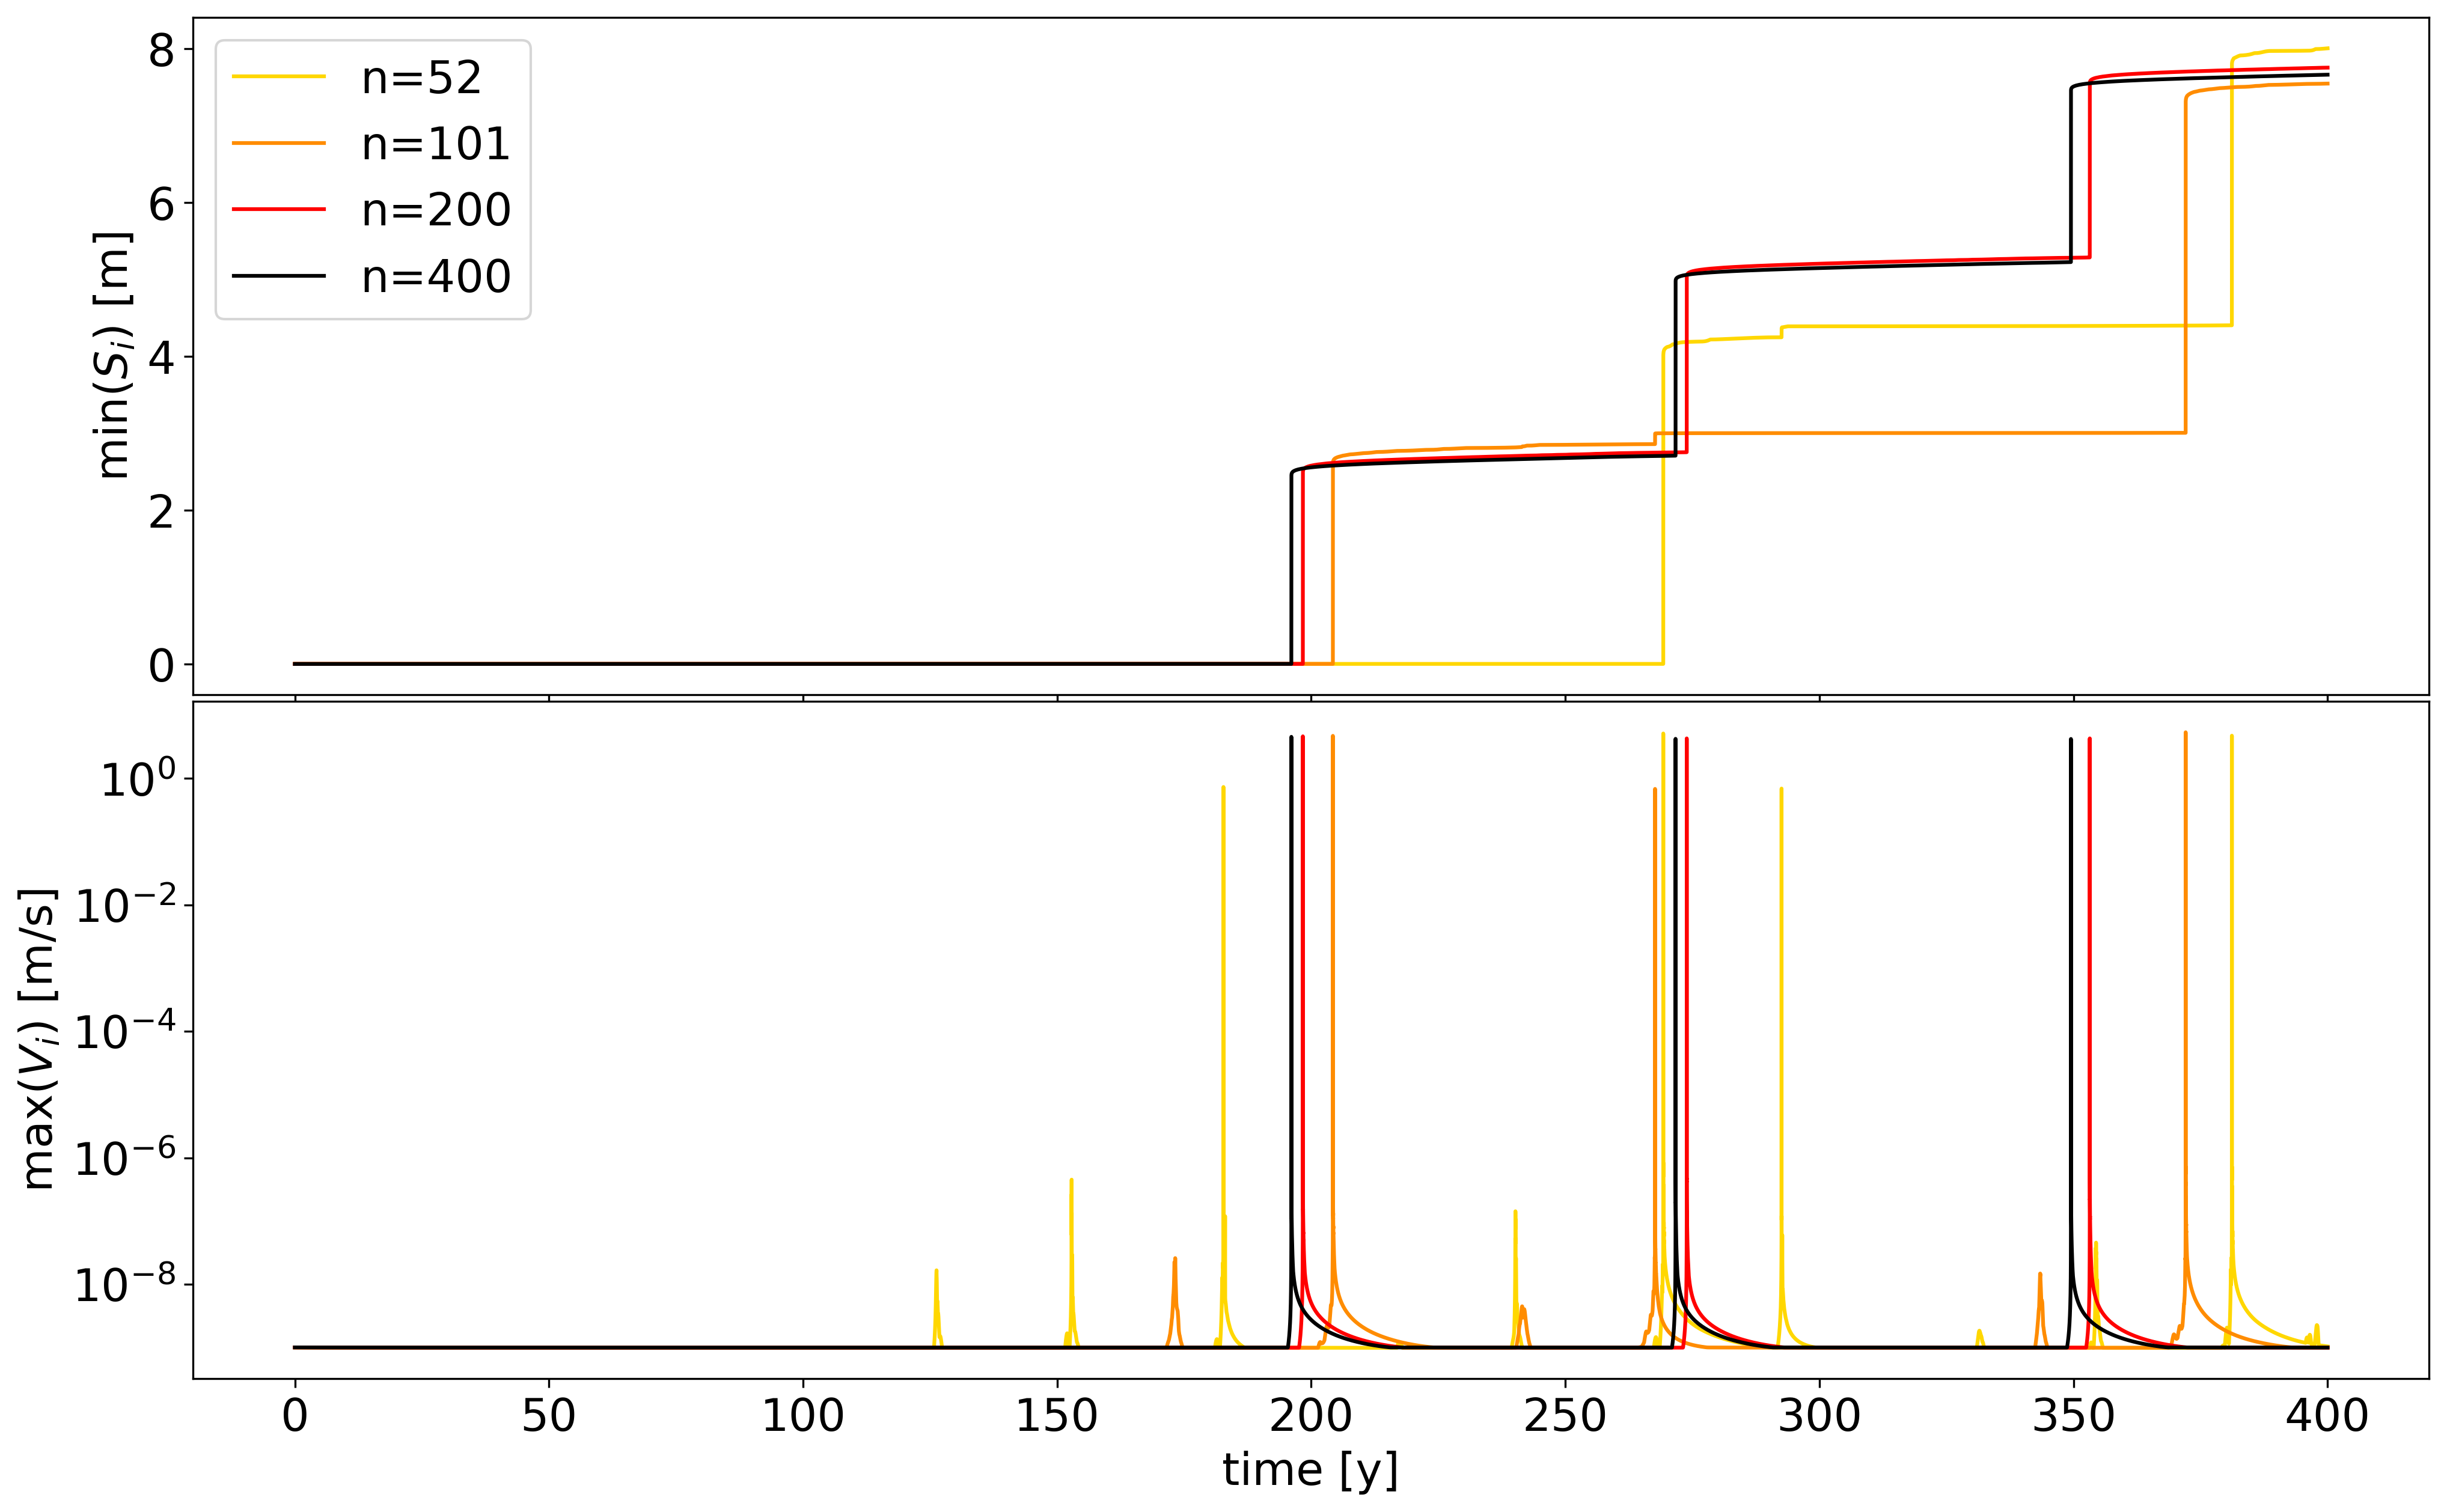
\includegraphics[width=0.7\textwidth]{images/TANDEMtimeEvolution_2D_scalability_extendedODE_RK.png}
	\caption{Evolution of the minimum slip $S$ and of the maximum slip rate $V$ over 400 years on a domain for different fault resolutions with $n$ fault elements.}
	\label{fig:EvolutionAllQuantitiesScalability}
\end{figure}

 \noindent ing fault resolutions. For coarse meshes, the slip rate has many peaks that are not associated with a significant increase in slip; these are falsely detected earthquakes and can only be avoided with finer meshes. Moreover, the coarser the mesh is, the later and stronger the earthquake develops. Only with 200 and 400 fault elements exclusively real earthquakes are detected, but they are still delayed by two and a half years on average. For each earthquake, the slip advance is slightly different and the interseismic period is longer, as the third earthquake occurs delayed by almost four years. For longer simulations, the results of fine and coarse mesh resolutions would further diverge, this is why a high spatial resolution is fundamental for accurate SEAS simulations. \\


As this thesis focuses on time integration and not on the spatial domain discretization, this issue is mentioned here, but not further investigated in later discussions.
